\documentclass[border=6pt]{standalone}
\usepackage{tikz}
\usetikzlibrary{arrows.meta,positioning,decorations.pathreplacing}
\usepackage{amsmath,amssymb}

\definecolor{CornellRed}{RGB}{179,27,27}

\begin{document}
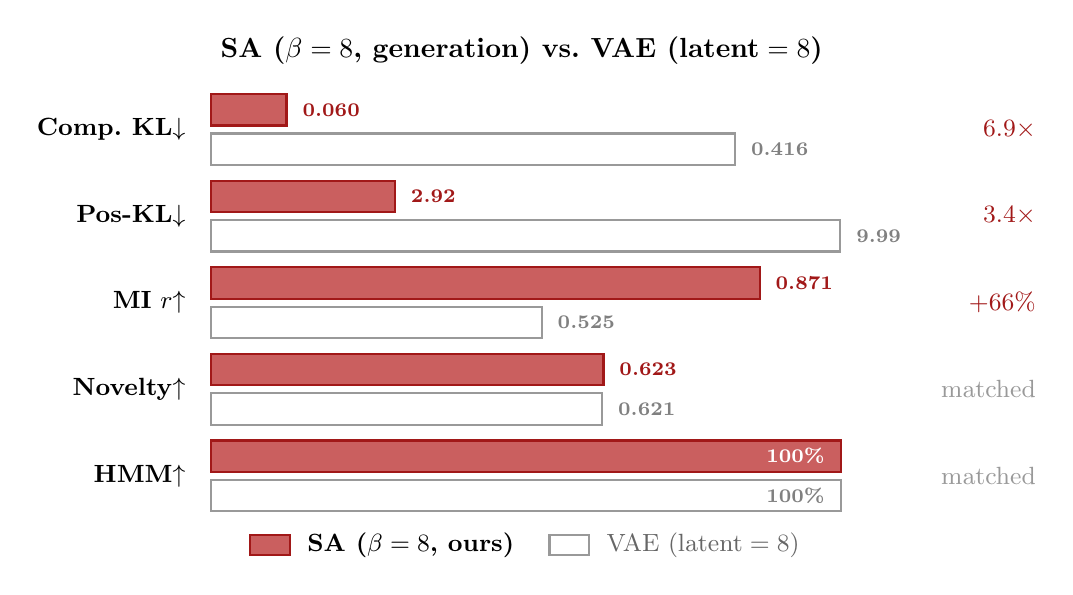
\begin{tikzpicture}

\def\chartx{0.0}
\def\charty{0.0}
\def\barh{0.20}
\def\gap{0.05}
\def\maxbar{8.0}
\def\labelx{10.6}  % right-aligned edge for all annotations

% Title
\node[font=\normalsize\bfseries, anchor=south west] at (\chartx, \charty+0.5) {SA ($\beta=8$, generation) vs.\ VAE (latent${}=8$)};

% --- Metric 1: Global KL ---
\def\mone{\charty-0.2}
\node[font=\small, anchor=east] at (\chartx-0.2, \mone) {\textbf{Comp.\ KL}$\downarrow$};
% SA bar (top)
\fill[CornellRed!70] (\chartx, \mone+\gap) rectangle (\chartx+0.96, \mone+\gap+2*\barh);
\draw[thick, CornellRed!90!black] (\chartx, \mone+\gap) rectangle (\chartx+0.96, \mone+\gap+2*\barh);
\node[font=\scriptsize\bfseries, CornellRed!90!black, anchor=west] at (\chartx+0.96+0.08, \mone+\gap+\barh) {0.060};
% VAE bar (bottom)
\fill[white] (\chartx, \mone-\gap-2*\barh) rectangle (\chartx+6.656, \mone-\gap);
\draw[thick, black!40] (\chartx, \mone-\gap-2*\barh) rectangle (\chartx+6.656, \mone-\gap);
\node[font=\scriptsize\bfseries, black!50, anchor=west] at (\chartx+6.656+0.08, \mone-\gap-\barh) {0.416};
\node[font=\small\bfseries, CornellRed!90!black, anchor=east] at (\labelx, \mone) {$6.9\times$};

% --- Metric 2: Per-position KL ---
\def\mtwo{\charty-1.3}
\node[font=\small, anchor=east] at (\chartx-0.2, \mtwo) {\textbf{Pos-KL}$\downarrow$};
\fill[CornellRed!70] (\chartx, \mtwo+\gap) rectangle (\chartx+2.336, \mtwo+\gap+2*\barh);
\draw[thick, CornellRed!90!black] (\chartx, \mtwo+\gap) rectangle (\chartx+2.336, \mtwo+\gap+2*\barh);
\node[font=\scriptsize\bfseries, CornellRed!90!black, anchor=west] at (\chartx+2.336+0.08, \mtwo+\gap+\barh) {2.92};
\fill[white] (\chartx, \mtwo-\gap-2*\barh) rectangle (\chartx+7.992, \mtwo-\gap);
\draw[thick, black!40] (\chartx, \mtwo-\gap-2*\barh) rectangle (\chartx+7.992, \mtwo-\gap);
\node[font=\scriptsize\bfseries, black!50, anchor=west] at (\chartx+7.992+0.08, \mtwo-\gap-\barh) {9.99};
\node[font=\small\bfseries, CornellRed!90!black, anchor=east] at (\labelx, \mtwo) {$3.4\times$};

% --- Metric 3: MI correlation ---
\def\mthree{\charty-2.4}
\node[font=\small, anchor=east] at (\chartx-0.2, \mthree) {\textbf{MI}~$r$$\uparrow$};
\fill[CornellRed!70] (\chartx, \mthree+\gap) rectangle (\chartx+6.968, \mthree+\gap+2*\barh);
\draw[thick, CornellRed!90!black] (\chartx, \mthree+\gap) rectangle (\chartx+6.968, \mthree+\gap+2*\barh);
\node[font=\scriptsize\bfseries, CornellRed!90!black, anchor=west] at (\chartx+6.968+0.08, \mthree+\gap+\barh) {0.871};
\fill[white] (\chartx, \mthree-\gap-2*\barh) rectangle (\chartx+4.2, \mthree-\gap);
\draw[thick, black!40] (\chartx, \mthree-\gap-2*\barh) rectangle (\chartx+4.2, \mthree-\gap);
\node[font=\scriptsize\bfseries, black!50, anchor=west] at (\chartx+4.2+0.08, \mthree-\gap-\barh) {0.525};
\node[font=\small\bfseries, CornellRed!90!black, anchor=east] at (\labelx, \mthree) {$+66\%$};

% --- Metric 4: Novelty ---
\def\mfour{\charty-3.5}
\node[font=\small, anchor=east] at (\chartx-0.2, \mfour) {\textbf{Novelty}$\uparrow$};
\fill[CornellRed!70] (\chartx, \mfour+\gap) rectangle (\chartx+4.984, \mfour+\gap+2*\barh);
\draw[thick, CornellRed!90!black] (\chartx, \mfour+\gap) rectangle (\chartx+4.984, \mfour+\gap+2*\barh);
\node[font=\scriptsize\bfseries, CornellRed!90!black, anchor=west] at (\chartx+4.984+0.08, \mfour+\gap+\barh) {0.623};
\fill[white] (\chartx, \mfour-\gap-2*\barh) rectangle (\chartx+4.968, \mfour-\gap);
\draw[thick, black!40] (\chartx, \mfour-\gap-2*\barh) rectangle (\chartx+4.968, \mfour-\gap);
\node[font=\scriptsize\bfseries, black!50, anchor=west] at (\chartx+4.968+0.08, \mfour-\gap-\barh) {0.621};
\node[font=\small, black!40, anchor=east] at (\labelx, \mfour) {matched};

% --- Metric 5: HMM pass ---
\def\mfive{\charty-4.6}
\node[font=\small, anchor=east] at (\chartx-0.2, \mfive) {\textbf{HMM}$\uparrow$};
\fill[CornellRed!70] (\chartx, \mfive+\gap) rectangle (\chartx+\maxbar, \mfive+\gap+2*\barh);
\draw[thick, CornellRed!90!black] (\chartx, \mfive+\gap) rectangle (\chartx+\maxbar, \mfive+\gap+2*\barh);
\node[font=\scriptsize\bfseries, white, anchor=east] at (\chartx+\maxbar-0.08, \mfive+\gap+\barh) {100\%};
\fill[white] (\chartx, \mfive-\gap-2*\barh) rectangle (\chartx+\maxbar, \mfive-\gap);
\draw[thick, black!40] (\chartx, \mfive-\gap-2*\barh) rectangle (\chartx+\maxbar, \mfive-\gap);
\node[font=\scriptsize\bfseries, black!50, anchor=east] at (\chartx+\maxbar-0.08, \mfive-\gap-\barh) {100\%};
\node[font=\small, black!40, anchor=east] at (\labelx, \mfive) {matched};

% Legend
\fill[CornellRed!70] (\chartx+0.5, \charty-5.6) rectangle (\chartx+1.0, \charty-5.35);
\draw[thick, CornellRed!90!black] (\chartx+0.5, \charty-5.6) rectangle (\chartx+1.0, \charty-5.35);
\node[font=\small\bfseries, anchor=west] at (\chartx+1.1, \charty-5.475) {SA ($\beta=8$, ours)};

\fill[white] (\chartx+4.3, \charty-5.6) rectangle (\chartx+4.8, \charty-5.35);
\draw[thick, black!40] (\chartx+4.3, \charty-5.6) rectangle (\chartx+4.8, \charty-5.35);
\node[font=\small, black!60, anchor=west] at (\chartx+4.9, \charty-5.475) {VAE (latent${}=8$)};

\end{tikzpicture}
\end{document}
